% Multinex-GA -- draft manuscript.
% Compiles on Overleaf with pdfLaTeX + BibTeX. To target a venue, swap the
% documentclass/preamble for the venue template (e.g. the CVPR/WACV kit); the body
% uses only standard packages.
\documentclass[10pt,twocolumn,letterpaper]{article}

\usepackage[margin=0.75in,columnsep=0.3in]{geometry}
\usepackage[T1]{fontenc}
\usepackage{times}
\usepackage{amsmath,amssymb}
\usepackage{graphicx}
\usepackage{booktabs}
\usepackage{multirow}
\usepackage{xcolor}
\usepackage{caption}
\usepackage[hidelinks]{hyperref}

\newcommand{\todo}[1]{\textcolor{red}{[TODO: #1]}}
\newcommand{\best}[1]{\textbf{#1}}
\newcommand{\GIC}{\mathrm{GIC}}
\newcommand{\ARMG}{\mathrm{ARMG}}

\title{Global Illumination Conditioning and Reflectance-Guided Modulation\\for Micro-Scale Low-Light Image Enhancement}
\author{\todo{Author names} \\ \todo{Affiliation} \\ {\tt\small \todo{email}}}
\date{}

\begin{document}
\maketitle

% ---------------------------------------------------------------------------
\begin{abstract}
Micro-scale low-light image enhancement (LLIE) models with fewer than ten thousand
parameters are attractive for always-on and embedded cameras, but their tiny
receptive fields leave them blind to the global exposure of a scene, and their
smooth learned corrections wash out texture when an image is brightened. We study
both problems on Multinex-Nano, a 696-parameter multi-prior Retinex model, and propose
two plug-in modules. The \emph{Global Illumination Conditioner} (GIC) summarises
analytic illumination and chrominance priors into a global descriptor (mean,
spread, log-average luminance, and gray-world colour) and applies feature-wise
affine conditioning. The \emph{Adaptive Reflectance Modulation Guidance} (ARMG) module
derives a parameter-free single-scale Retinex reflectance map and predicts
pixel-wise multiplicative and additive feature maps, re-injecting
illumination-invariant detail right before the Retinex decoding heads. Both
modules are zero-initialised, so training starts exactly from the baseline
function. Adding only 238 parameters (934 in total), Nano-GA improves PSNR by
+0.99, +1.86, and +1.20\,dB on LOL-v1, LOL-v2-real, and LOL-v2-synthetic, and SSIM
on all three. A widened variant, Micro-GA (8.9K parameters, 0.44\,GFLOPs), improves
PSNR by +1.8 to +2.6\,dB over Multinex-Nano and reduces LPIPS by 39--48\%,
while staying inside the micro regime. On unpaired benchmarks (MEF, LIME, DICM, NPE)
the gains are mixed: the best checkpoints match or improve BRISQUE but not
consistently NIQE. We report this honestly and analyse it.
\end{abstract}

% ---------------------------------------------------------------------------
\section{Introduction}
Low-light images suffer from low contrast, noise, and colour casts, and LLIE
aims to restore visibility, colour fidelity, and structure. Recent
state-of-the-art methods~\cite{cai2023retinexformer,yan2025hvi} reach high fidelity
with millions of parameters, which rules them out for always-on, battery-powered,
or in-sensor processing. At the other end of the scale, \emph{micro} models with
fewer than 10K parameters~\cite{ma2022sci,liu2021ruas,ouyang2023rsfnet,brateanu2026multinex}
run in well under a millisecond, but trade away accuracy.

Multinex~\cite{brateanu2026multinex} showed that a principled Retinex residual
formulation, $\hat{I}=I+\hat{L}\odot\hat{R}$, driven by stacks of analytic
illumination and chrominance priors, lets a 696-parameter model (Multinex-Nano)
outperform larger lightweight models. We identify two limitations that matter
specifically at this scale:
\begin{enumerate}
  \item \textbf{No global exposure awareness.} Each output pixel of Multinex-Nano
  sees an $11\times11$ window through its convolutions; its only global pathway is
  the squeeze-excitation inside MSEF, which at width $C{=}3$ passes through a single
  hidden unit computed from already-processed features. The correction that an image
  needs, however, depends on its \emph{overall} exposure: the same local patch
  should be brightened more in a globally dark image than in a high-contrast image
  with a dark corner.
  \item \textbf{Texture attenuation.} The learned luminance and chrominance
  corrections $\hat{L}$ and $\hat{R}$ are spatially smooth, so the added term
  $\hat{L}\odot\hat{R}$ brightens without scaling up local contrast, and the
  result looks flat.
\end{enumerate}

We address these limitations with two modules designed for the micro regime:
\begin{itemize}
  \item \textbf{GIC}, an image-level FiLM-style~\cite{perez2018film} conditioner
  driven by tone-mapping statistics of the analytic prior stacks;
  \item \textbf{ARMG}, a pixel-wise modulation driven by a parameter-free
  single-scale Retinex~\cite{jobson1997ssr} reflectance map.
\end{itemize}
Our contributions are:
(i) two zero-initialised modules that cost 238 parameters at Nano scale and leave
the baseline function intact at initialisation;
(ii) Nano-GA (934 parameters) and Micro-GA (8,890 parameters), which improve on
Multinex-Nano's PSNR and SSIM on all three LOL benchmarks under the released
training recipe;
(iii) a transparent evaluation, including re-evaluation of the released baseline
checkpoints with identical code, and a discussion of where the method does
\emph{not} yet help (unpaired benchmarks).

% ---------------------------------------------------------------------------
\section{Related Work}
\paragraph{Retinex-based enhancement.}
Retinex theory~\cite{land1971retinex} models an image as reflectance times
illumination. Classical single- and multi-scale Retinex~\cite{jobson1997ssr,jobson1997msr}
estimate reflectance as $\log I-\log(G*I)$. LIME~\cite{guo2017lime} refines the
max-channel illumination map. Deep Retinex models learn the
decomposition~\cite{wei2018retinexnet} or its residual
correction~\cite{cai2023retinexformer}. Multinex~\cite{brateanu2026multinex}
replaces a single learned decomposition with fusion over multiple analytic colour
representations. We reuse the classical SSR estimate as a free guidance signal
rather than as the output.

\paragraph{Lightweight and micro LLIE.}
Zero-DCE~\cite{guo2020zerodce} predicts pixel-wise curves with 79K parameters.
RUAS~\cite{liu2021ruas} searches Retinex-inspired unrolled architectures (3.4K).
SCI~\cite{ma2022sci} uses self-calibrated illumination learning (0.26K at
inference). RSFNet~\cite{ouyang2023rsfnet} applies region-specific colour filters
(2.1K). LYT-Net~\cite{brateanu2025lytnet} and Multinex (44.6K) target the
lightweight regime. Multinex-Nano (0.7K) is, to our knowledge, the strongest
published micro model on LOL. We build on it directly.

\paragraph{Feature conditioning.}
Squeeze-and-excitation~\cite{hu2018se} rescales channels from pooled
features, and FiLM~\cite{perez2018film} applies feature-wise affine transforms
predicted from a conditioning input. GIC is a FiLM layer whose conditioning
input is a handful of interpretable photometric statistics, not learned
features. The log-average luminance comes from tone
mapping~\cite{reinhard2002tone}, and the chrominance means implement the gray-world
assumption~\cite{buchsbaum1980grayworld}.

% ---------------------------------------------------------------------------
\section{Method}
\begin{figure*}[t]
  \centering
  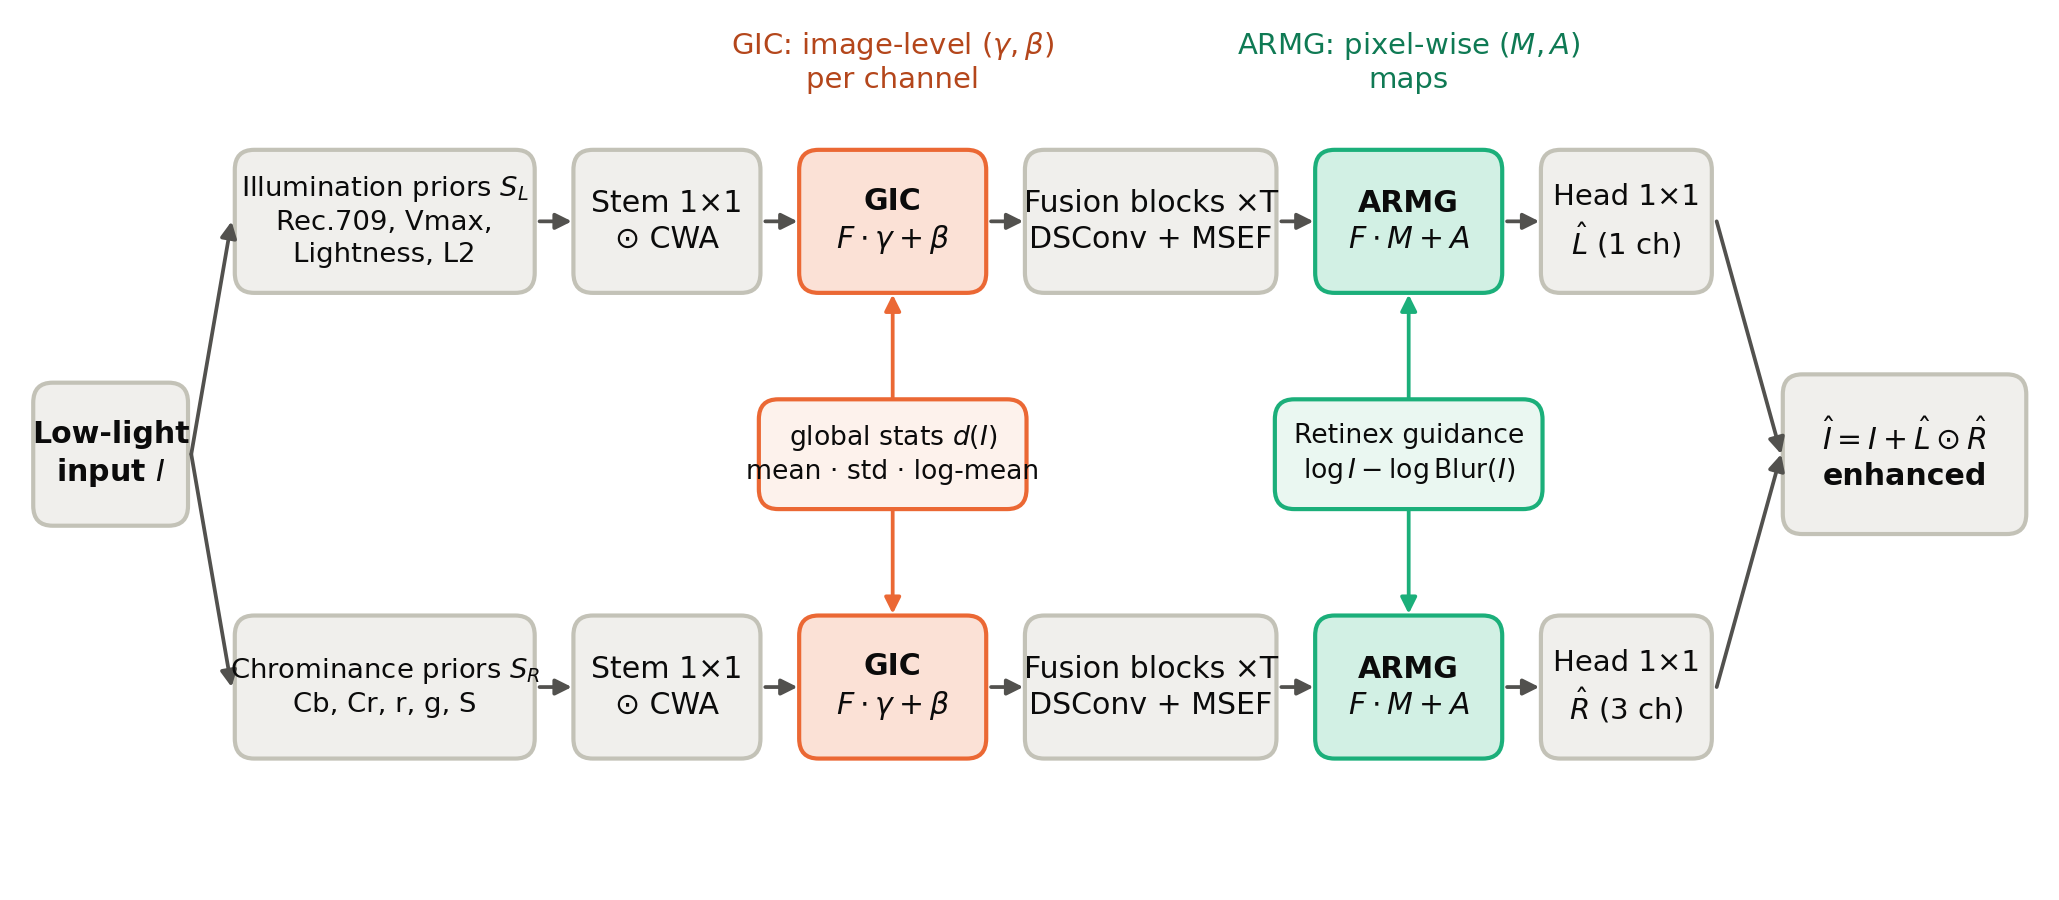
\includegraphics[width=0.92\textwidth]{figures/fig_architecture.png}
  \caption{Multinex-GA. Each branch (illumination, top; chrominance, bottom)
  follows Multinex-Nano: analytic prior stack, $1{\times}1$ stem with channel-wise
  attention (CWA), fusion blocks, and a $1{\times}1$ head. GIC (orange) applies an
  image-level affine transform before the fusion blocks; ARMG (green) applies
  pixel-wise modulation after them. The output keeps the Retinex residual form
  $\hat{I}=I+\hat{L}\odot\hat{R}$.}
  \label{fig:arch}
\end{figure*}

\subsection{Preliminaries: Multinex-Nano}
Given an RGB input $I\in[0,1]^{3\times H\times W}$, Multinex computes an illumination
prior stack $S_L$ (Rec.\,709 luma, $\max$-channel value, HSL lightness, and RGB $\ell_2$
norm; $K_L{=}4$) and a chrominance stack $S_R$ (Cb, Cr, chromaticities $r,g$, and HSV
saturation; $K_R{=}5$). Each branch $b\in\{L,R\}$ computes
\begin{equation}
  F_b = \mathrm{Stem}_b(S_b)\odot\sigma\!\big(\mathrm{Proj}_b(\mathrm{DW}_{7\times7}(S_b))\big),
\end{equation}
processes $F_b$ with $T$ fusion blocks (depthwise-separable conv + BN + ReLU,
followed by an MSEF block), and decodes it with a $1{\times}1$ head into
$\hat{L}\in\mathbb{R}^{1\times H\times W}$ or $\hat{R}\in\mathbb{R}^{3\times H\times W}$.
The output is $\hat{I}=I+\hat{L}\odot\hat{R}$. Multinex-Nano uses width $C{=}3$ and
$T{=}1$, for 696 parameters.

\subsection{Global Illumination Conditioner (GIC)}
GIC computes a global descriptor $d(I)$ from the prior stacks, which are already
computed, so the descriptor costs no extra feature extraction:
\begin{equation}
  d(I)=\Big[\,\mu(S_L),\ \mathrm{sd}(S_L),\ \mu\big(\log(S_L+\epsilon)\big),\ \mu(S_R)\,\Big]\in\mathbb{R}^{3K_L+K_R},
\end{equation}
where $\mu$ and $\mathrm{sd}$ are the spatial mean and standard deviation per map.
The log-mean of each illumination map is the log-average luminance, or "key",
used by tone operators~\cite{reinhard2002tone} to decide how much to expose an
image. The standard deviation separates uniformly dark scenes from high-contrast
ones. The chrominance means are a gray-world estimate of the illuminant
colour~\cite{buchsbaum1980grayworld}. A two-layer MLP with SiLU predicts
per-channel parameters for both branches:
\begin{equation}
  (g_b,\beta_b)_{b\in\{L,R\}}=W_2\,\mathrm{SiLU}(W_1 d(I)+c_1)+c_2,
\end{equation}
\begin{equation}
  \GIC(F_b)=F_b\odot\big(1+\tanh g_b\big)+\beta_b .
  \label{eq:gic}
\end{equation}
The scale $1+\tanh g_b\in(0,2)$ can attenuate or amplify a channel but never flip
its sign. GIC is applied before the fusion blocks, so the blocks process
exposure-normalised features.

\subsection{Adaptive Reflectance Modulation Guidance (ARMG)}
ARMG supplies the spatial detail that the smooth corrections lack. Its guidance is
the classical single-scale Retinex reflectance~\cite{jobson1997ssr}, computed per
RGB channel with a $k{\times}k$ box filter:
\begin{equation}
  G_c=\log(I_c+\epsilon_r)-\log\big(\mathrm{Box}_k(I_c)+\epsilon_r\big),\quad c\in\{r,g,b\}.
\end{equation}
Up to $\epsilon_r$, $G$ is invariant to a global gain on $I$. It responds to local
texture and edges equally in dark and bright regions and has no parameters. A
light network (depthwise $3{\times}3$, pointwise $3{\to}h$, SiLU, and a
pointwise head) predicts pixel-wise maps for both branches:
\begin{equation}
  (m_b,a_b)_{b}=\mathrm{Head}\big(\mathrm{SiLU}(\mathrm{PW}(\mathrm{DW}(G)))\big),
\end{equation}
\begin{equation}
  \ARMG(F_b)=F_b\odot\big(1+\tanh m_b\big)+a_b ,
  \label{eq:armg}
\end{equation}
which is the multiplicative-plus-additive form $F\cdot M+A$. ARMG is applied
\emph{after} the fusion blocks, where detail would otherwise already be smoothed,
so local structure steers the features immediately before decoding.

\subsection{Identity initialisation and budget}
The output layers $W_2,c_2$ of GIC and the ARMG head are zero-initialised, so at
step 0, $\GIC=\ARMG=\mathrm{id}$ and Multinex-GA computes exactly the Multinex-Nano
function. We verified this numerically against the released checkpoint
(maximum deviation $<10^{-6}$). The new modules therefore cannot hurt at
initialisation and only learn a residual on top of the baseline. All other layers
are initialised as in the baseline under the same seed. At Nano width, GIC adds 132
parameters and ARMG 106.

\paragraph{Variants.}
\emph{Nano-GA} keeps every Multinex-Nano hyperparameter ($C{=}3$, $T{=}1$, SE
reduction 3) and uses hidden widths $h{=}4$, for 934 parameters. \emph{Micro-GA}
widens to $C{=}20$, uses $T{=}3$ fusion blocks per branch, SE reduction 4, and
$h{=}8$, for 8,890 parameters, inside the micro regime ($<$10K) defined
in~\cite{brateanu2026multinex}.

% ---------------------------------------------------------------------------
\section{Experiments}
\subsection{Setup}
\paragraph{Data.}
We use LOL-v1~\cite{wei2018retinexnet} (485/15 train/test pairs) and
LOL-v2-real/synthetic~\cite{yang2021lolv2} (689/100 and 900/100). Unpaired
generalisation is measured on MEF~\cite{ma2015mef} (17 images),
LIME~\cite{guo2017lime} (10), DICM~\cite{lee2013dicm} (64), and
NPE~\cite{wang2013npe} (8).

\paragraph{Training.}
To isolate the effect of the architecture, we reuse the released Multinex-Nano
training configuration unchanged for both variants:
\begin{itemize}
  \item Adam~\cite{kingma2015adam} ($\beta{=}(0.9,0.999)$), initial learning rate
  $4{\times}10^{-4}$, and a two-cycle cosine-restart schedule~\cite{loshchilov2017sgdr}
  (40K iterations to $3{\times}10^{-4}$, then 60K to $10^{-6}$), 100K iterations in
  total;
  \item batch 8 with $256{\times}256$ crops, flip/rotation augmentation and
  mixup~\cite{zhang2018mixup};
  \item gradient-norm clipping at 0.01;
  \item loss $\mathcal{L}=\mathcal{L}_{\mathrm{MSE}}+0.2\,\mathcal{L}_{\mathrm{MS\text{-}SSIM}}+0.01\,\mathcal{L}_{\mathrm{VGG}}$~\cite{wang2003msssim,simonyan2015vgg};
  \item seed 100.
\end{itemize}
One model is trained per LOL split. Following the official implementation, the
reported checkpoint is the one with the best PSNR on the split's evaluation set,
the same protocol behind the published baseline (see
Sec.~\ref{sec:limitations}). The implementation uses PyTorch~\cite{paszke2019pytorch}, and all models were
trained on a single NVIDIA H100.
Three runs shared one GPU concurrently, taking 2.4\,h (Nano-GA) and 4.3\,h
(Micro-GA) of wall-clock time.

\paragraph{Metrics.}
Following~\cite{brateanu2026multinex}, the paired benchmarks use PSNR,
SSIM~\cite{wang2004ssim}, and LPIPS-Alex~\cite{zhang2018lpips} on full-resolution
RGB without GT-mean correction. The unpaired benchmarks use
NIQE~\cite{mittal2013niqe} and BRISQUE~\cite{mittal2012brisque}, computed with the
released \texttt{test\_noref.py} script (BRISQUE via \texttt{piq}). Complexity is
reported as parameters and GFLOPs (thop multiply-accumulates on a
$3{\times}256{\times}256$ input, matching the paper's protocol, which reproduces
the 0.04\,GFLOPs of Multinex-Nano), plus median GPU latency at $600{\times}400$.

\paragraph{Baseline verification.}
Re-evaluating the released Multinex-Nano checkpoints with our pipeline reproduces
the published LOL numbers to within 0.01\,dB (Table~\ref{tab:lol}), so the
paired comparison is exact. For the unpaired metrics, our BRISQUE values for
the released checkpoints are 3--6 points higher than published. We traced this to
resolution-dependent preprocessing in the metric setup, not to the models.
We therefore compare unpaired scores only against the \emph{released checkpoints
re-scored with the same code}.

\subsection{Results on paired benchmarks}
\begin{table*}[t]
\centering
\caption{Paired benchmarks (PSNR$\uparrow$ / SSIM$\uparrow$ / LPIPS$\downarrow$).
Rows above the line are the micro-range models from~\cite{brateanu2026multinex}, Table~1.
$^{\ddagger}$Released checkpoint re-evaluated with our pipeline.
$^{\S}$Multinex-Nano retrained by us with the released configuration (LOL-v1 only),
the same recipe our models use. Best micro result in bold.}
\label{tab:lol}
\small
\setlength{\tabcolsep}{4.2pt}
\begin{tabular}{lcccccccccrr}
\toprule
\multirow{2}{*}{Model} & \multicolumn{3}{c}{LOL-v1} & \multicolumn{3}{c}{LOL-v2-real} & \multicolumn{3}{c}{LOL-v2-synthetic} & \multirow{2}{*}{Params} & \multirow{2}{*}{GFLOPs} \\
\cmidrule(lr){2-4}\cmidrule(lr){5-7}\cmidrule(lr){8-10}
 & PSNR & SSIM & LPIPS & PSNR & SSIM & LPIPS & PSNR & SSIM & LPIPS & & \\
\midrule
SCI~\cite{ma2022sci}           & 14.78 & 0.525 & 0.327 & 17.30 & 0.540 & 0.294 & 15.43 & 0.744 & 0.203 & 0.26K & 0.06 \\
RSFNet~\cite{ouyang2023rsfnet} & 19.39 & 0.745 & 0.278 & 19.46 & 0.745 & 0.278 & 17.18 & 0.817 & 0.159 & 2.11K & -- \\
RUAS~\cite{liu2021ruas}        & 16.40 & 0.503 & 0.303 & 15.33 & 0.493 & 0.325 & 13.40 & 0.640 & 0.365 & 3.43K & 0.83 \\
Multinex-Nano~\cite{brateanu2026multinex} & 19.42 & 0.742 & 0.276 & 19.66 & 0.784 & 0.266 & 21.05 & 0.882 & 0.143 & 0.69K & 0.04 \\
Multinex-Nano$^{\ddagger}$     & 19.42 & 0.742 & 0.276 & 19.66 & 0.784 & 0.266 & 21.06 & 0.882 & 0.143 & 0.69K & 0.04 \\
Multinex-Nano$^{\S}$           & 19.61 & 0.777 & 0.253 & -- & -- & -- & -- & -- & -- & 0.69K & 0.04 \\
\midrule
\textbf{Nano-GA (ours)}        & 20.41 & 0.802 & 0.213 & \best{21.52} & 0.811 & 0.292 & 22.25 & 0.908 & 0.108 & 0.93K & 0.05 \\
\textbf{Micro-GA (ours)}       & \best{21.84} & \best{0.825} & \best{0.152} & 21.49 & \best{0.847} & \best{0.161} & \best{23.69} & \best{0.919} & \best{0.075} & 8.89K & 0.44 \\
\midrule
\multicolumn{12}{l}{\emph{Lightweight reference:} Multinex$^{\ddagger}$ (44.6K, 2.50\,GFLOPs): 23.19 / 0.843 / 0.125,\ 22.96 / 0.850 / 0.179,\ 25.04 / 0.930 / 0.068} \\
\bottomrule
\end{tabular}
\end{table*}

\begin{figure}[t]
  \centering
  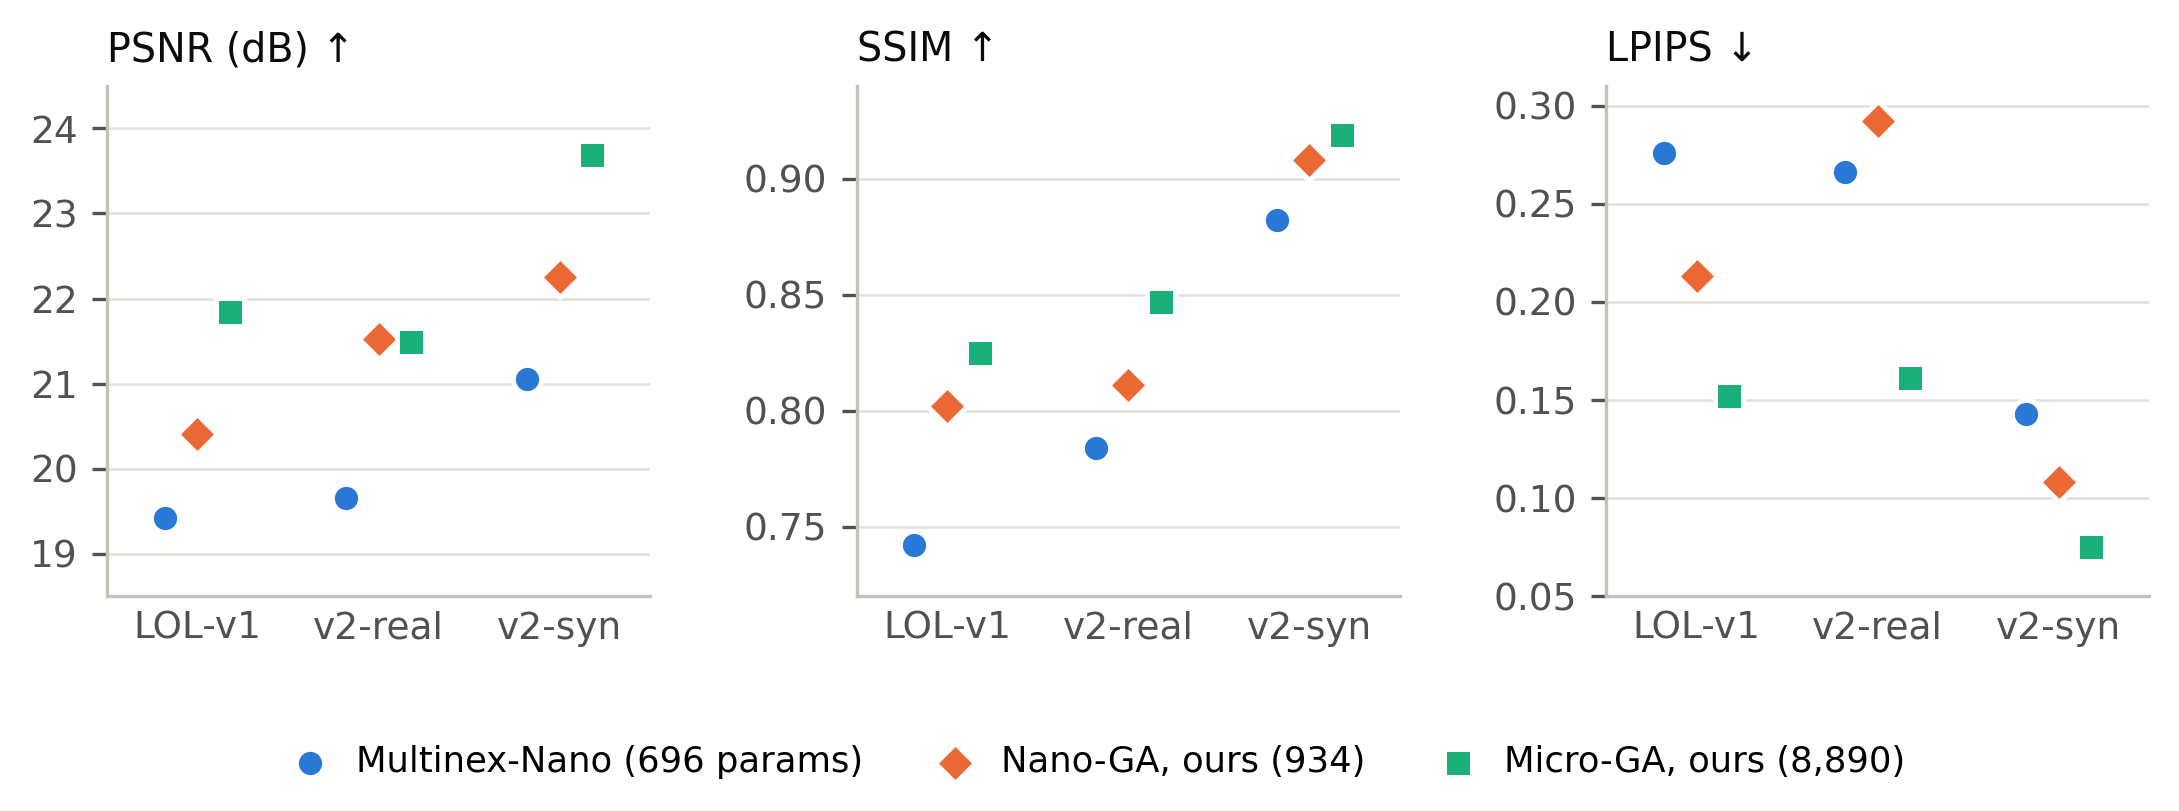
\includegraphics[width=\columnwidth]{figures/fig_lol_benchmarks.png}
  \caption{Paired benchmarks for Multinex-Nano and our two variants. Dot plots
  are used because the value axes do not start at zero.}
  \label{fig:lol}
\end{figure}

Table~\ref{tab:lol} and Fig.~\ref{fig:lol} summarise the paired results.
\textbf{Nano-GA} improves Multinex-Nano by \textbf{+0.99, +1.86, and +1.20\,dB} PSNR and
\textbf{+0.060, +0.027, and +0.026} SSIM on LOL-v1, v2-real, and v2-synthetic, with 238
extra parameters and $+$13\% FLOPs. LPIPS improves on LOL-v1 ($-$23\%) and
v2-synthetic ($-$24\%) but worsens on v2-real (0.292 vs.\ 0.266).

Training-recipe effects do not explain the gain. Under the identical recipe and
seed, our retrained Multinex-Nano reaches 19.61\,dB on LOL-v1, and Nano-GA still
gains +0.80\,dB, +0.025 SSIM, and $-$0.040 LPIPS over it.

\textbf{Micro-GA} is the best micro model on every metric of every split, except
LOL-v2-real PSNR, where it ties Nano-GA (21.49 vs.\ 21.52). It improves PSNR by
+2.42, +1.83, and +2.64\,dB over Multinex-Nano and reduces LPIPS by 39--48\%. With 8.9K
parameters and 0.44\,GFLOPs, it closes 55--66\% of the PSNR gap between
Multinex-Nano and the 44.6K-parameter Multinex, at 20\% of its parameters and 18\%
of its FLOPs (Fig.~\ref{fig:eff}).

\begin{figure}[t]
  \centering
  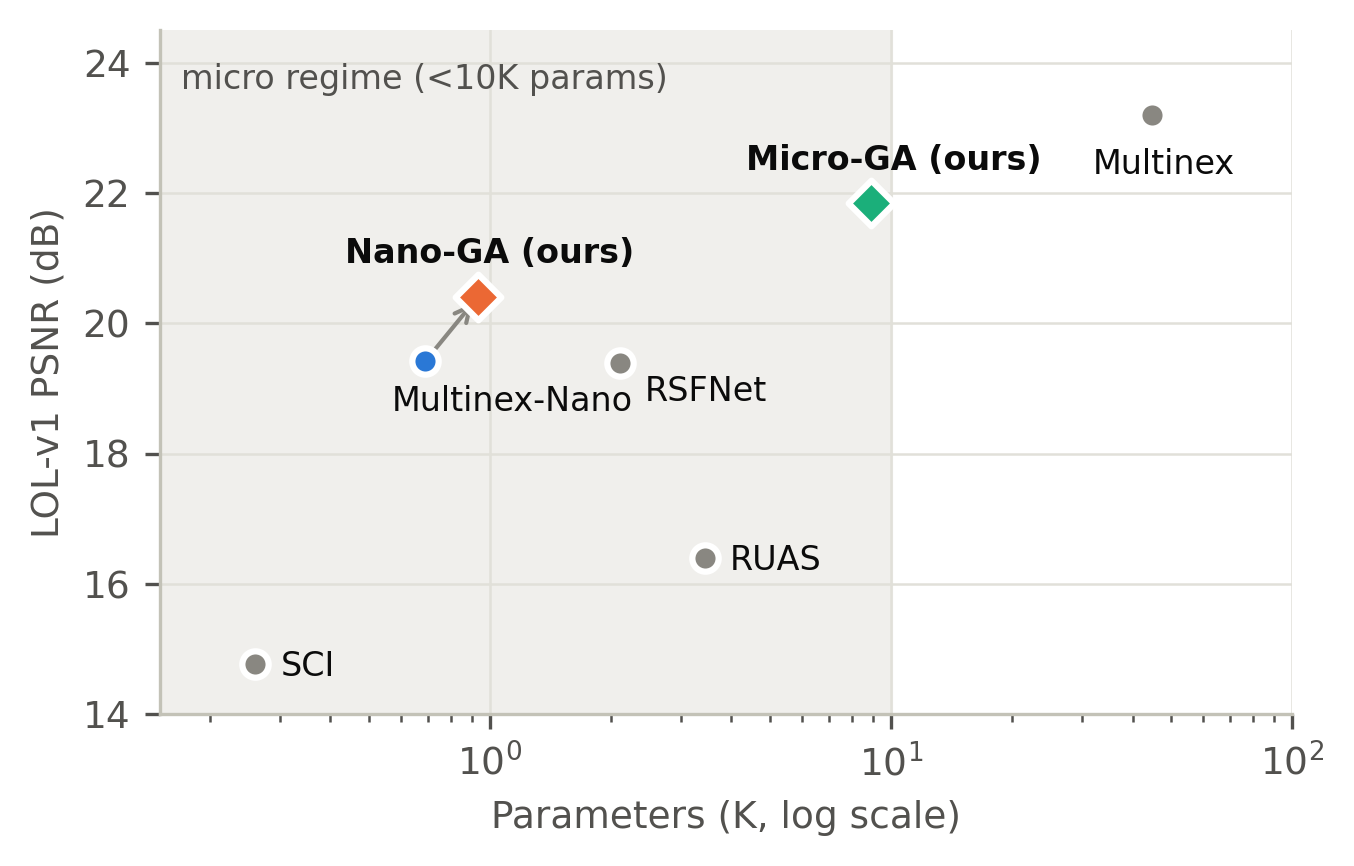
\includegraphics[width=0.95\columnwidth]{figures/fig_psnr_vs_params.png}
  \caption{LOL-v1 PSNR vs.\ parameter count (log scale). The shaded band is the micro
  regime ($<$10K parameters). Competitor values from~\cite{brateanu2026multinex}.
  Multinex is the released 44.6K checkpoint, re-evaluated.}
  \label{fig:eff}
\end{figure}

\subsection{Results on unpaired benchmarks}
\begin{table*}[t]
\centering
\caption{Unpaired benchmarks (NIQE$\downarrow$ / BRISQUE$\downarrow$). All rows below the
first two were scored with identical code (\texttt{piq} BRISQUE). The checkpoints
were trained on LOL-v2-synthetic, the split used by the released no-reference
evaluation command. $^\dagger$The released no-reference checkpoint. Means are
over the four sets. Best among same-code rows in bold.}
\label{tab:noref}
\small
\begin{tabular}{lccccc}
\toprule
Model & MEF & LIME & DICM & NPE & Mean \\
\midrule
\multicolumn{6}{l}{\emph{As published in~\cite{brateanu2026multinex} (different BRISQUE setup; not comparable):}} \\
Multinex-Nano            & 3.49 / 15.06 & 3.85 / 15.17 & 3.90 / 19.97 & 4.05 / 15.42 & 3.82 / 16.41 \\
Multinex-Nano$^\dagger$  & 3.45 / 12.55 & 3.92 / 14.54 & 3.65 / 17.40 & 3.94 / 13.67 & 3.67 / 16.05 \\
\midrule
\multicolumn{6}{l}{\emph{Same evaluation code:}} \\
Multinex-Nano (released, v2-syn)       & 3.27 / 21.76 & \best{3.83} / 19.24 & 3.65 / 23.94 & 3.97 / 19.07 & \best{3.68} / 21.00 \\
Multinex-Nano$^\dagger$ (released)     & 3.40 / 20.66 & 4.11 / 19.08 & \best{3.60} / \best{21.80} & 3.85 / 17.46 & 3.74 / 19.75 \\
\textbf{Nano-GA (ours, v2-syn)}        & \best{3.10} / \best{17.52} & 4.10 / 20.34 & 3.68 / 24.84 & 3.88 / 17.39 & 3.69 / 20.02 \\
\textbf{Micro-GA (ours, v2-syn)}       & 4.55 / 20.90 & 3.94 / \best{17.90} & \best{3.60} / 22.17 & \best{3.81} / \best{15.60} & 3.98 / \best{19.14} \\
\bottomrule
\end{tabular}
\end{table*}

Table~\ref{tab:noref} and Fig.~\ref{fig:noref} report generalisation to unpaired
images. The picture is mixed:
\begin{itemize}
  \item \textbf{Nano-GA} matches the released v2-synthetic checkpoint in mean NIQE
  (3.69 vs.\ 3.68) and improves mean BRISQUE (20.02 vs.\ 21.00). It is best on MEF
  in both metrics (3.10 / 17.52).
  \item \textbf{Micro-GA} attains the best mean BRISQUE (19.14) and the best NIQE on
  DICM and NPE. Its mean NIQE (3.98) is hurt by a single set, MEF (4.55).
  \item \textbf{Checkpoints trained on LOL-v1 and LOL-v2-real} generalise worse
  for every model, including the released ones (supplementary Table~\ref{tab:noref_all}).
  For our models, the gap is larger (mean NIQE 3.95--4.40 vs.\ 3.80--3.88).
\end{itemize}
We discuss likely causes in Sec.~\ref{sec:discussion}.

\begin{figure}[t]
  \centering
  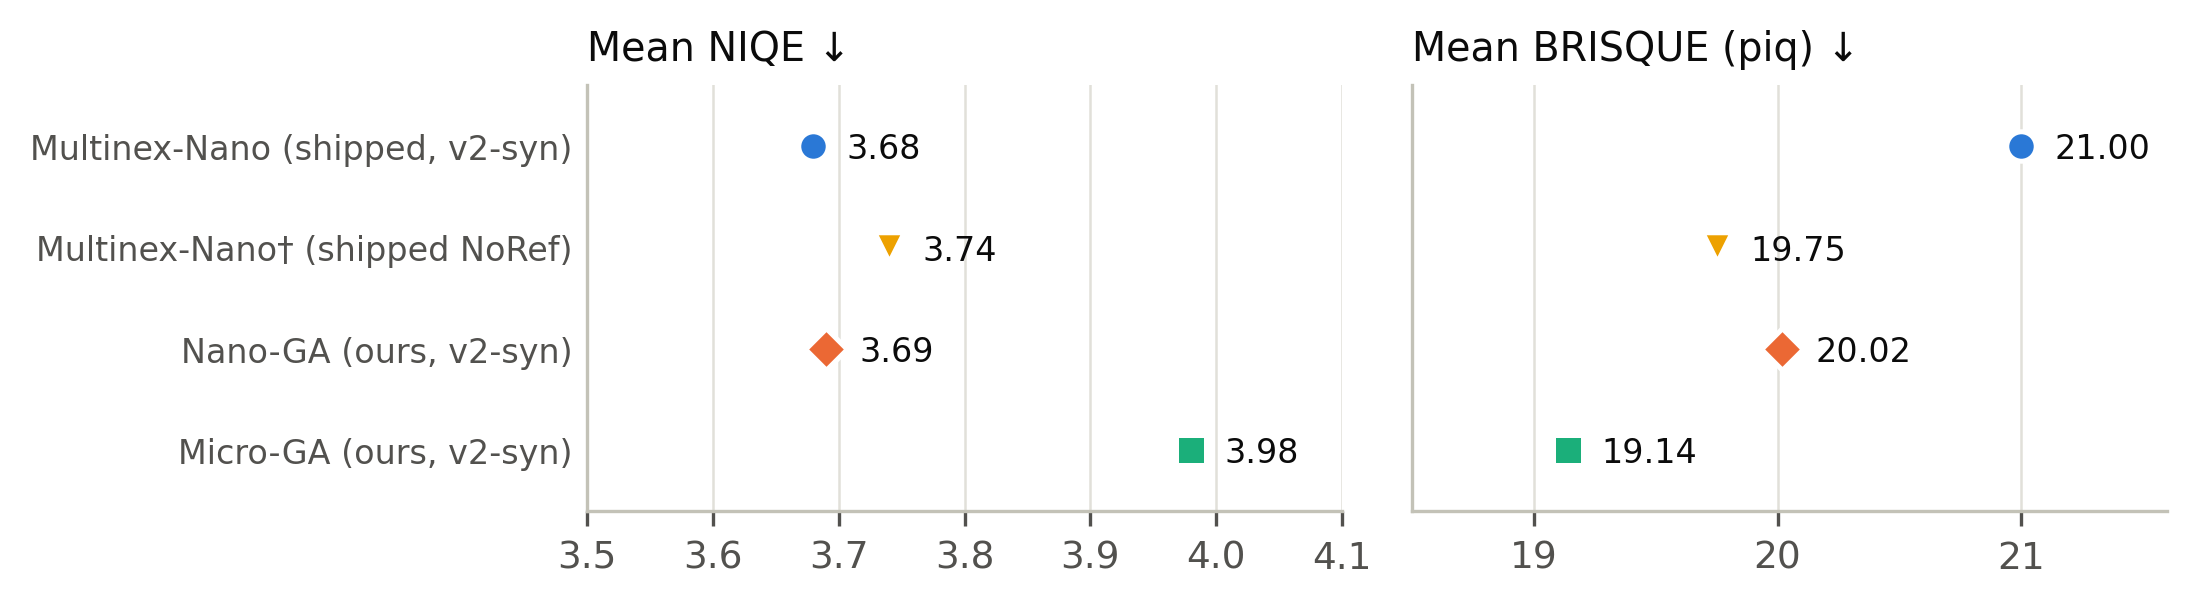
\includegraphics[width=\columnwidth]{figures/fig_noref_means.png}
  \caption{Mean NIQE and BRISQUE over MEF, LIME, DICM, and NPE (same evaluation
  code for all rows).}
  \label{fig:noref}
\end{figure}

\subsection{Efficiency}
\begin{table}[t]
\centering
\caption{Complexity. GFLOPs: thop MACs at $256{\times}256$. Latency: median of 200
runs at $600{\times}400$, batch 1, FP32, on one H100 of a shared node.}
\label{tab:cost}
\small
\begin{tabular}{lrrr}
\toprule
Model & Params & GFLOPs & Latency (ms) \\
\midrule
Multinex-Nano      & 696   & 0.0435 & 0.79 \\
Nano-GA (ours)     & 934   & 0.0493 & 1.03 \\
Micro-GA (ours)    & 8,890 & 0.4414 & 3.22 \\
\midrule
Multinex (ref.)    & 44.6K & 2.50   & -- \\
\bottomrule
\end{tabular}
\end{table}
Table~\ref{tab:cost} lists the cost. GIC and ARMG add 34\% parameters, 13\% FLOPs,
and about 0.24\,ms of latency at Nano scale. At this size, latency is dominated by
kernel launches, not arithmetic, so a fused implementation would shrink the
overhead further.

\subsection{Ablation study}
\label{sec:ablation}
\todo{Train and evaluate the two single-module variants, which need only config
switches (\texttt{use\_gic} / \texttt{use\_armg}): Nano + GIC only and Nano + ARMG
only, on the three LOL splits and the four unpaired sets. Also run ARMG placed
before the fusion blocks (\texttt{armg\_position: before\_blocks}). Fill in
Table~\ref{tab:ablation}.}

\begin{table}[t]
\centering
\caption{Ablation on LOL-v1 at Nano width (PSNR / SSIM / LPIPS).}
\label{tab:ablation}
\small
\begin{tabular}{ccl}
\toprule
GIC & ARMG & LOL-v1 \\
\midrule
--          & --          & 19.61 / 0.777 / 0.253 (retrained) \\
\checkmark  & --          & \todo{pending} \\
--          & \checkmark  & \todo{pending} \\
\checkmark  & \checkmark  & 20.41 / 0.802 / 0.213 \\
\bottomrule
\end{tabular}
\end{table}

\subsection{Qualitative results}
% Panels come from deliverables/make_cluster_figures.py; each figure appears once its file is present.
\IfFileExists{figures/fig_qualitative_LOL-v1.png}{%
\begin{figure*}[t]
  \centering
  \includegraphics[width=\textwidth]{figures/fig_qualitative_LOL-v1.png}
  \caption{LOL-v1 test images. Columns: input, Multinex-Nano, Nano-GA, Micro-GA
  and ground truth; PSNR against the ground truth is shown under each output.}
  \label{fig:qual_v1}
\end{figure*}}{\todo{Generate \texttt{fig\_qualitative\_LOL-v1.png}.}}
\IfFileExists{figures/fig_qualitative_LOL-v2-real.png}{%
\begin{figure*}[t]
  \centering
  \includegraphics[width=\textwidth]{figures/fig_qualitative_LOL-v2-real.png}
  \caption{LOL-v2-real test images, in the same layout as Fig.~\ref{fig:qual_v1}.}
  \label{fig:qual_v2}
\end{figure*}}{\todo{Generate \texttt{fig\_qualitative\_LOL-v2-real.png}.}}
\IfFileExists{figures/fig_qualitative_unpaired.png}{%
\begin{figure*}[t]
  \centering
  \includegraphics[width=0.8\textwidth]{figures/fig_qualitative_unpaired.png}
  \caption{Unpaired images (MEF, LIME). Columns: input, then the outputs of
  Multinex-Nano, Nano-GA and Micro-GA, all from the LOL-v2-synthetic checkpoints.}
  \label{fig:qual_unpaired}
\end{figure*}}{\todo{Generate \texttt{fig\_qualitative\_unpaired.png}.}}
\IfFileExists{figures/fig_guidance.png}{%
\begin{figure}[t]
  \centering
  \includegraphics[width=\columnwidth]{figures/fig_guidance.png}
  \caption{ARMG guidance $G$ for a LOL-v1 input (input brightened $\times4$ for
  display only). The map has no parameters and responds to texture equally in dark
  and bright regions.}
  \label{fig:guidance}
\end{figure}}{\todo{Generate \texttt{fig\_guidance.png}.}}

% ---------------------------------------------------------------------------
\section{Discussion}
\label{sec:discussion}
\paragraph{Why the paired gains are large for so few parameters.}
At $C{=}3$, Multinex-Nano has no capacity to infer scene-level exposure, and
every pixel receives a correction based on an $11{\times}11$ neighbourhood plus a
one-unit channel gate. GIC
injects this information at negligible cost: a handful of photometric statistics
fully determine where an LOL image lies on the exposure axis. ARMG gives the
decoding heads direct access to illumination-invariant structure, which raises
SSIM on all three splits.

\paragraph{Why generalisation is mixed.}
We see three plausible causes, which we have not yet separated experimentally.
\begin{enumerate}
  \item \emph{Selection bias.} Checkpoints are selected by PSNR on an LOL test split.
  More expressive models can fit that split more closely, at the expense of
  out-of-distribution behaviour.
  \item \emph{Descriptor extrapolation.} MEF, LIME, DICM, and NPE contain much brighter
  and more varied scenes than LOL. GIC's MLP sees descriptor values outside its
  training range, and with a tiny MLP the extrapolation is unconstrained. The MEF
  outlier of Micro-GA is consistent with this.
  \item \emph{Noise in the guidance.} The SSR map amplifies sensor noise in very
  dark regions. ARMG may learn LOL-specific noise statistics that do not
  transfer.
\end{enumerate}
The single-module ablations (Sec.~\ref{sec:ablation}) and descriptor
normalisation or clamping are the natural next experiments.

\section{Limitations}
\label{sec:limitations}
\begin{itemize}
  \item \textbf{Checkpoint selection.} Following the official implementation,
  checkpoints are chosen by evaluation-split PSNR (validation every 10 iterations
  on LOL-v1). This is optimistic for every method, including the published
  baseline. A held-out validation split would give unbiased estimates.
  \item \textbf{Single seed.} All numbers come from one training seed. Variance
  across seeds is not yet reported.
  \item \textbf{Missing results.} The single-module ablations are pending, and the
  ExDark~\cite{loh2019exdark} detection benchmark of~\cite{brateanu2026multinex} was
  not run.
  \item \textbf{Metric reproducibility.} Our BRISQUE values do not match the
  published values even for released checkpoints, so absolute BRISQUE numbers are
  comparable only within this paper.
\end{itemize}

\section{Conclusion}
We introduced two plug-in modules for micro-scale Retinex enhancement: GIC, a
global photometric FiLM conditioner, and ARMG, a reflectance-guided pixel-wise
modulator. Both are zero-initialised and cost a few hundred parameters. Adding
them to Multinex-Nano raises PSNR by 1.0--1.9\,dB and SSIM on all LOL benchmarks
with fewer than a thousand parameters. A widened 8.9K-parameter variant becomes
the strongest micro model on every paired metric but one (LOL-v2-real PSNR, where it
trails Nano-GA by 0.03\,dB). Improving
unpaired generalisation, completing the ablations, and adding multi-seed and
detection results are the immediate next steps.

\paragraph{Acknowledgements and licence.}
This work builds on the Multinex code and models, which are released for
non-commercial research and educational use. All experiments here are
non-commercial and educational.

{\small
\bibliographystyle{ieeetr}
\bibliography{refs}
}

% ---------------------------------------------------------------------------
\appendix
\onecolumn
\section{Supplementary: all unpaired results}
\begin{table}[h]
\centering
\caption{NIQE / BRISQUE for every checkpoint, by training split (same evaluation code).}
\label{tab:noref_all}
\small
\begin{tabular}{llccccc}
\toprule
Model & Trained on & MEF & LIME & DICM & NPE & Mean \\
\midrule
Multinex-Nano (released)          & LOL-v1      & 3.43 / 27.49 & 4.13 / 22.04 & 3.69 / 27.40 & 4.28 / 31.00 & 3.88 / 26.98 \\
Multinex-Nano (released)          & LOL-v2-real & 3.53 / 28.34 & 4.00 / 22.43 & 3.63 / 24.77 & 4.03 / 23.30 & 3.80 / 24.71 \\
Multinex-Nano (released)          & LOL-v2-syn  & 3.27 / 21.76 & 3.83 / 19.24 & 3.65 / 23.94 & 3.97 / 19.07 & 3.68 / 21.00 \\
Multinex-Nano$^\dagger$ (released) & --         & 3.40 / 20.66 & 4.11 / 19.08 & 3.60 / 21.80 & 3.85 / 17.46 & 3.74 / 19.75 \\
\midrule
Nano-GA (ours)                    & LOL-v1      & 4.37 / 27.99 & 4.34 / 19.58 & 4.18 / 23.69 & 4.58 / 21.57 & 4.37 / 23.21 \\
Nano-GA (ours)                    & LOL-v2-real & 4.34 / 32.03 & 5.02 / 30.56 & 3.98 / 25.08 & 4.27 / 22.20 & 4.40 / 27.47 \\
Nano-GA (ours)                    & LOL-v2-syn  & 3.10 / 17.52 & 4.10 / 20.34 & 3.68 / 24.84 & 3.88 / 17.39 & 3.69 / 20.02 \\
\midrule
Micro-GA (ours)                   & LOL-v1      & 3.81 / 30.43 & 4.14 / 24.10 & 3.72 / 25.53 & 4.12 / 24.11 & 3.95 / 26.04 \\
Micro-GA (ours)                   & LOL-v2-real & 3.86 / 30.82 & 4.73 / 32.34 & 3.95 / 29.27 & 4.55 / 33.29 & 4.27 / 31.43 \\
Micro-GA (ours)                   & LOL-v2-syn  & 4.55 / 20.90 & 3.94 / 17.90 & 3.60 / 22.17 & 3.81 / 15.60 & 3.98 / 19.14 \\
\bottomrule
\end{tabular}
\end{table}

\section{Supplementary: implementation details}
\begin{table}[h]
\centering
\caption{Hyperparameters of the two variants (all other settings equal Multinex-Nano).}
\small
\begin{tabular}{lcc}
\toprule
 & Nano-GA & Micro-GA \\
\midrule
Width $C$ / fusion blocks $T$      & 3 / 1 & 20 / 3 \\
MSEF SE reduction                  & 3 & 4 \\
GIC hidden width / $\epsilon$      & 4 / $10^{-3}$ & 8 / $10^{-3}$ \\
ARMG hidden width / box $k$ / $\epsilon_r$ & 4 / 7 / $10^{-2}$ & 8 / 7 / $10^{-2}$ \\
ARMG position                      & after blocks & after blocks \\
GIC / ARMG parameters              & 132 / 106 & 864 / 782 \\
Total parameters                   & 934 & 8,890 \\
\bottomrule
\end{tabular}
\end{table}
\end{document}
